\begin{defi}[Operador de Laplace]
Seja $f$ uma função duplamente derivável de valores reais no espaço euclidiano $\mathbb{R}^n$. O \textbf{operador de Laplace} (também conhecido como Laplaciano), denotado por $\Delta$ ou $\nabla^2$, é definido como o divergente do gradiente:
\begin{equation}
\Delta f = \nabla^2 f = \nabla \cdot (\nabla f) = \text{div} (\text{grad f})
\end{equation}
\end{defi}

A denominação de \textbf{operador de Laplace-Beltrami} vem no contexto de geometria diferencial, em que o Laplaciano pode ser generalizado para operar sobre funções definidas em subvariedades no espaço euclideano e, mais genericamente, em variedades Riemannianas e pseudo-Riemannianas.

\begin{defi}[Coordenadas diferenciais]
	Seja uma malha triangular de $n$ vértices caracterizada por $\mathcal{M} = (V, E, F)$, em que $V, A, F$ são, respectivamente, os conjuntos de seus vértices, arestas e faces. Cada vértice $\mathbf{v}_i \in V$ possui uma representação cartesiana dada por $\mathbf{v}_i = (x_i,y_i,z_i)$. \textbf{Coordenadas diferenciais} (também conhecidas como $\mathbf{\delta}$\textit{-coordenadas}) de $\mathbf{v}_i$ são definidas como a diferença entre a coordenada cartesiana e o centro de massa de seus vizinhos imediatos na malha:
	
	\begin{equation}
	\mathbf{\delta}_i = (\mathbf{\delta}_i^{(x)}, \mathbf{\delta}_i^{(y)}, \mathbf{\delta}_i^{(z)}) = \mathbf{v}_i - \frac{1}{d_i} \sum_{j \in N(i)} \mathbf{v}_j,
	\label{eq_delta}
	\end{equation}
	
	\noindent em que $N(i) = \{j|(i,j) \in E$\} (ou seja, os vértices adjacentes a $i$) e $d_i = |N(i)|$ é o número dos vizinhos imediatos de $i$ (grau de $i$).
\end{defi}

A transformação do vetor de coordenadas cartesianas absolutas ao vetor das $\mathbf{\delta}$-coordenadas, descrita na equação \ref{eq_delta}, também pode ser representada em forma de matriz. Seja $A$ a matriz de adjacências da malha:

\begin{equation}\label{eqMatAdj}
A_{ij} = \begin{cases}
1&(i, j) \in E\\
0&\text{caso contrário.}
\end{cases}
\end{equation}

\noindent e $D$ matriz diagonal tal que $D_{ii} = d_i$ (grau de incidência do nó $i$). Assim, a matriz transformação de coordenadas absolutas para as coordenadas relativas é:

\begin{equation}
L = I - D^{-1}A.
\end{equation}

É mais conveniente utilizar a versão simétrica $L_s$ da matriz $L$, definida por:

\begin{equation}\label{eqMatLaplaciana}
L_s = DL = D - A
\end{equation}

\noindent em que cada célula pode ser calculada da seguinte forma:

\begin{equation}
(L_s)_{ij} = \begin{cases}
d_i&i=j\\
-1&(i, j) \in E\\
0&\text{caso contrário.}
\end{cases}
\end{equation}

A matriz $L_s$ é denominada \textit{Laplaciano topológico} da malha $\mathcal M$. A figura \ref{fig:matrizLaplaciana} ilustra um exemplo de uma simples malha triangular e sua respectiva representação matricial Laplaciana.

\begin{figure}[htb]
	\centering
	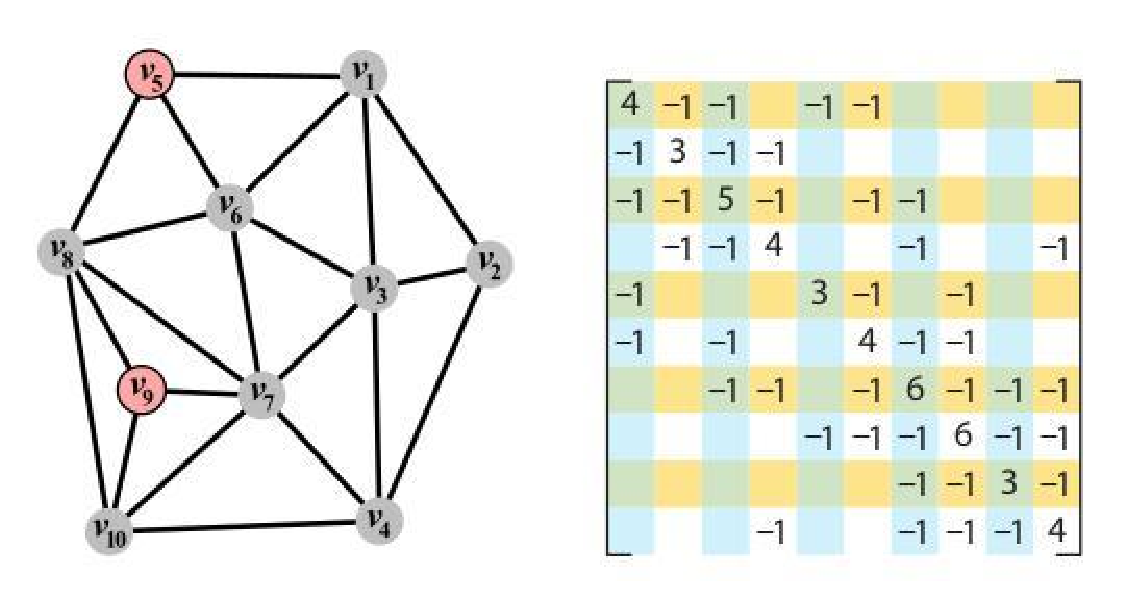
\includegraphics[width=.5\linewidth]{imagens/cap4/meshLaplacian.eps}
	\caption{Uma malha triangular e sua respectiva matriz Laplaciana $L_s$ \cite{sorkine2006}}
	\label{fig:matrizLaplaciana}
\end{figure}

Caso a malha $\mathcal{M}$ seja a aproximação linear por partes de uma superfície suave, as $\mathbf{\delta}$-coordenadas podem ser vistas como a discretização do operador contínuo de Laplace-Beltrami. Pode-se denotar o vetor de coordenadas diferenciais em um vértice $v_i$ como

\begin{equation}
\mathbf{\delta}_i = \frac{1}{d_i} \sum_{j \in N(i)} (\mathbf{v}_i - \mathbf{v}_j)
\end{equation}

\noindent em que este somatório é a discretização da seguinte integral:

\begin{equation}
\frac{1}{|\gamma|} \int_{\mathbf{v} \in \gamma} (\mathbf{v}_i - v) dl(\mathbf{v}))
\end{equation}

\noindent onde $\gamma$ é uma superfície simples e fechada em torno de $\mathbf{v}$ e $|\gamma|$ é o comprimento de $\gamma$. Sabe-se que

\begin{equation}
	\lim_{|\gamma| \rightarrow 0} \frac{1}{|\gamma|} \int_{\mathbf{v} \in \gamma} (\mathbf{v}_i - \mathbf{v}) dl(\mathbf{v}) =  -H(\mathbf{v}_i)\mathbf{n}_i
\end{equation}


\noindent em que $H(\mathbf{v}_i)$ é a curvatura média em $\mathbf{v}_i$ e $\mathbf{n}_i$ é o vetor normal à superfície. Assim, a direção do vetor de coordenadas diferenciais aproxima a direção normal e sua norma aproxima a quantidade proporcional à curvatura média local (o vetor normal escalado pela curvatura média é dito normal da curvatura média). Intuitivamente, isto significa que as $\mathbf{\delta}$-coordenadas encapsulam a forma da superfície local.

Portanto, como ilustra a figura \ref{fig:coordDif}, as coordenadas diferenciais aproximam não apenas as características da forma local da superfície, mas também a direção normal e a curvatura média. 

\begin{figure}[htb]
	\centering
	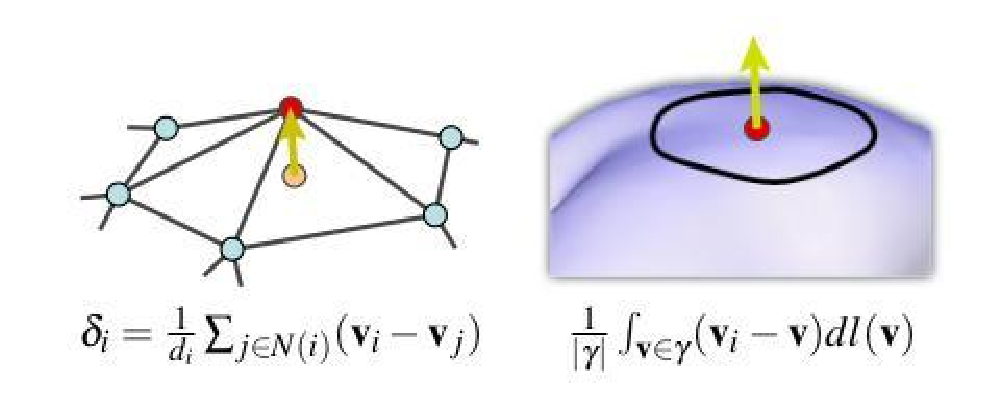
\includegraphics[width=.7\linewidth]{imagens/cap4/difcoord.eps}
	\caption{O vetor da coordenada diferencial em um vértice aproxima a forma local superfície: representação da direção normal e da curvatura média \cite{sorkine2006}}
	\label{fig:coordDif}
\end{figure}

Existem outras formas de se calcular as $\delta$-coordenadas, de forma a se obter melhores qualidades de aproximação. Por exemplo, pode-se ponderar geometricamente o somatório com cotangentes \cite{pinkall:1996}:

\begin{equation}
	\mathbf{\delta}_i^c = \frac{1}{|\Omega|} \sum_{j \in N(i)} \frac{1}{2} (\cot \alpha_{ij} + \cot \beta_{ij})(\mathbf{v}_i - \mathbf{v}_j))
\end{equation}

\noindent em que $|\Omega|$ é o tamanho da célula de Voronoi de $i$ e $\alpha_{ij}, \beta_{ij}$ são os dois ângulos opostos à aresta $(i, j)$. Esta ponderação gera os vetores $\mathbf{\delta}_i^c$, que possuem apenas componentes normais (ao contrário das $\mathbf{\delta}$-coordenadas definidas anteriormente, que podem possuir componentes tangenciais e serem não nulas em 1-anéis planares). Porém, os valores das cotangentes podem ser negativos ou possuírem alguns problemas (em ângulos com valores se aproximando de $\pi$).
